
当接受了某些数据共享即将发生的事实,就必须接受对共享数据的同步。记住,在没有同步的情况下,对相同数据的并发访问都会导致数据竞争和未定义行为。

保护共享数据的常用方法是使用互斥锁:

\begin{lstlisting}[style=styleCXX]
std::mutex m;
size_t count;// Guarded by m
… on the threads …
{
	std::lock_guard l(m);
	++count;
}
\end{lstlisting}

这里使用C++17模板类型推断来实现\texttt{std::lock\_guard}。在C++14中,必须指定模板类型实参。

使用互斥对象相当简单,访问共享数据的代码都应该位于临界区,也就是在锁定和解锁互斥对象的调用之间。互斥锁的实现有正确的内存栅栏,以确保临界区中的代码不会被硬件或编译器移出临界区(编译器通常不会在锁操作中移动代码。不过,只要遵循内存栅栏的语义,理论上可以做这样的优化)。

这时候通常会问的是:“互斥锁的开销有多大?”然而,这个问题并没有很好地答案:对于特定的硬件和给定的互斥锁实现,当然可以给出绝对的答案,甚至以纳秒为单位,但是这个值有什么意义呢?这当然比没有互斥对象开销小得多,但没有互斥对象,结果就会不正确(而且有更简单的方法可以快速生成不正确的程序)。所以,“开销大”的定义只能与替代方案相比较,这自然引出了下一个问题,替代方案是什么?

最明显的替代方法是使计数原子化:

\begin{lstlisting}[style=styleCXX]
std::atomic<size_t> count;
… on the threads …
++count;
\end{lstlisting}

还必须考虑需要什么内存序来与计数上的操作相关联。如果稍后使用该计数,例如在数组中进行下标索引,那可能需要释放-获取序。但如果只是一个计数,只是要统计一些事件并报告数量,那就不需要内存序限制:

\begin{lstlisting}[style=styleCXX]
std::atomic<size_t> count;
… on the threads …
count.fetch_add(1, std::memory_order_relaxed);
\end{lstlisting}

是否使用栅栏取决于硬件。在x86上,原子增量指令有“内置”的双向内存栅栏,自由序不会让它更快。尽管如此,为了可移植性和清晰性,指定代码需要的内存序仍然很重要。记住,\textbf{写代码不是给解析代码的编译器看的,而是给需要阅读代码的其他开发者看的}。

具有原子增量的程序没有锁,也不需要任何锁。然而,它依赖于特定的硬件能力。处理器有一个原子增量指令,这类指令的集合相当小。如果需要一个没有原子指令的操作,该怎么办?在C++中,没有原子乘法(不知道任何硬件有这样的能力。当然,在x86、ARM或其他任何通用CPU架构上都找不到)。

不过,有一种“通用的”原子操作,可以用来构建任何读-改-写操作(困难程度不同)。这个操作称为\textbf{比较-交换},在C++中称为\texttt{compare\_exchange}。它有两个参数:第一个是原子变量的预期当前值,第二个是预期的新值。如果实际的当前值与期望值不匹配,则什么也不会发生,原子变量也不会发生更改。但是,如果当前值与期望值匹配,则需要的值将写入原子变量。C++的\texttt{compare\_exchange}操作会返回true或false来指示写操作是否发生(如果发生则返回true)。如果变量与预期值不匹配,则在第一个参数中返回实际值。通过比较和交换,可以实现原子增量操作:

\begin{lstlisting}[style=styleCXX]
std::atomic<size_t> count;
… on the threads …
size_t c = count.load(std::memory_order_relaxed);
while (!count.compare_exchange_strong(c, c + 1,
	std::memory_order_relaxed, std::memory_order_relaxed)) {}
\end{lstlisting}

首先,C++中操作的实际名称是\texttt{compare\_exchange\_strong}和\texttt{compare\_exchange\_weak}。不同的是,即使当前值和期望值匹配,弱版本有时也会返回false(在x86上,这没有区别,但在一些平台上,弱版执行的更快)。其次,该操作接受两个内存序:第二个内存序应用于比较失败时(因此它只是操作的比较部分的内存顺序),第一个内存序应用于比较成功并发生写操作时。

分析这个实现是如何工作的。首先,以原子的方式读取count的当前值\texttt{c}。当然,增量后是\texttt{c + 1},但不能直接将其赋给count。因为在读取之后,更新之前,另一个线程也可以给count赋值。因此,必须进行条件写入:如果count的当前值仍然是\texttt{c},则将其替换为所需的值\texttt{c + 1}。否则,用新的当前值更新\texttt{c}(\texttt{compare\_exchange\_strong}可以做到),然后再试一次。只有捕捉到原子变量,在上次读取的时间和试图更新之间没有变化时,循环才会退出。当然,有原子增量操作时,就没有理由这样来增加计数。但这种方法可以推广到其他计算中,可以使用其他表达式,而不是\texttt{c + 1},并且程序将以同样的方式进行。

虽然这三个版本的代码都执行相同的操作,但它们之间有着根本性的区别,必须对此进行更详细的研究。

\subsubsubsection{6.3.1\hspace{0.2cm}锁、无锁和无等待}

使用互斥锁是最容易理解的,一个线程可以持有锁,因此线程可以增加计数。当释放锁后,另一个线程可以获取它并增加计数,依此类推。最多只能有一个线程持有锁并进行操作,所有需要访问的剩余线程都在等待该锁。但是,即使拥有锁的线程也不能保证可以正常运行。如果需要在完成任务之前访问另一个共享变量,那么可能需要等待由其他线程持有的锁。这是常见的基于锁的方式,通常不是最快的,但最容易理解。

第二种方式与第一种非常不同,进行原子增量操作的线程会毫不延迟地执行。当然,硬件本身必须锁定对共享数据的访问,以确保操作的原子性(这是通过一次对整个缓存线的独占访问,并授予一个处理器来实现的)。从开发者的角度来看,这种独占访问表明其本身会增加执行原子操作所需的时间。然而,代码本身没有等待,没有尝试和再尝试。这种程序称为\textbf{无等待}。在一个无等待程序中,所有线程都能正常运行,在任何时候都在执行操作(尽管线程之间为了访问同一个共享变量而发生争用,有些操作可能会花费更长的时间)。无等待的实现通常只适用于非常简单的操作(例如增加计数),但只要有这种实现,可能会比基于锁的实现更简单。

最后一个方式理解起来有些困难。这里没有锁,但有一个循环重复了未知的次数。这里的实现的功能类似于锁,任何等待锁的线程也会困在一个类似的循环中,不停的尝试获得锁。二者的关键的区别在于,基于锁的程序中,当一个线程获取锁失败,必须再次尝试时,可以推断其他线程拥有锁。不能确定线程是否会很快释放锁,或者其工作有什么进展(例如,可能正在等待用户输入一些东西)。在基于比较-交换的程序中,线程无法更新共享计数的唯一原因是其他线程先进行了更新。因此,在所有试图同时增加计数的线程中,至少有一个是成功的。这种程序称为\textbf{无锁}程序。

我们已经了解了并发程序主要的三种类型:

\begin{itemize}
\item 
无等待的程序中,每个线程都在执行必要的操作,并且总是朝着最终目标前进。不需要等待访问,也不需要重做任何工作。

\item 
无锁程序中,多个线程可能会更新相同的共享数据,但只有一个会成功。其余的将放弃基于原始值所做的工作,读取更新后的值,并再次进行计算。但至少有一个线程总是保证提交它的工作,而不必重做。因此,尽管不一定是全速前进,但整个程序是在前进的。

\item 
基于锁的程序中,线程持有使其能够访问共享数据的锁。但是,仅因为持有锁并不意味着会对这些数据做什么。因此,当并发访问发生时,最多只有一个线程在有进展,但这也无法保证。
\end{itemize}

理论上讲,这三个程序之间的区别很明显。但读者想知道,哪个版本更快?可以在谷歌基准测试中运行每个版本的代码。例如,下面是基于锁的版本:

\hspace*{\fill} \\ %插入空行
\noindent
\textbf{01\_sharing\_incr\_mbm.C}
\begin{lstlisting}[style=styleCXX]
std::mutex m;
size_t count = 0;
void BM_lock(benchmark::State& state) {
	if (state.thread_index == 0) count = 0;
	for (auto _ : state) {
		std::lock_guard l(m);
		++count;
	}
}
BENCHMARK(BM_lock)->Threads(2)->UseRealTime();
\end{lstlisting}

必须在线程之间共享的变量在全局作用域中声明。初始设置(如果有的话)可以限制为一个线程,其他基准也类似,只有测试的代码发生了变化。下面是结果:

%\hspace*{\fill} \\ %插入空行
\begin{center}
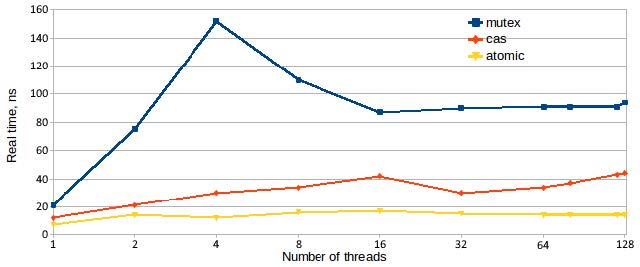
\includegraphics[width=0.9\textwidth]{content/2/chapter6/images/1.jpg}\\
图6.1 - 共享计数增量的性能:基于互斥锁、无锁(比较-交换,或CAS)和无等待(原子)
\end{center}

这里唯一想不到的结果是,基于锁的版本的性能非常差。然而,这只是一个数据点,并不是全部。特别是,虽然所有互斥对象都是锁,但并不是所有的锁都是互斥对象。可以尝试提出一种更有效的锁实现(至少,以满足我们的需求)。

\subsubsubsection{6.3.2\hspace{0.2cm}不同的问题使用不同的锁}

标准的C++互斥锁在保护对共享变量的访问时性能非常差,特别是当有很多线程在同一时间修改这个变量时(如果所有线程都在读取这个变量,根本不需要保护,并发只读访问不会导致数据竞争)。但是,锁的效率低下是因为实现,还是因为锁本身存在问题?根据前一章的了解,可以预期锁的效率都比原子递增计数器低,这是因为基于锁的方案会使用两个共享变量(锁和计数),而原子计数器只使用一个共享变量。然而,操作系统提供的互斥对象对于锁定非常短的操作(比如计数增量)通常不是特别有效。

对于这种情况,最简单有效的锁就是自旋锁。自旋锁的思想是:锁本身只是一个可以有两个值的标志,比如0和1。如果flag值为0,表示不锁定。看到这个值的线程都可以将标志设置为1并继续。当然,读取标志并将其设置为1的整个操作必须是原子操作。任何看到值为1的线程都必须等待,直到该值变回0,以表明锁可用。最后,当一个将标志从0更改为1的线程准备释放锁时,将把值更改回0。

锁实现的代码如下所示:

\begin{lstlisting}[style=styleCXX]
class Spinlock {
	public:
	void lock() {
		while (flag_.exchange(1, std::memory_order_acquire)) {}
	}
	void unlock() { flag_.store(0, std::memory_order_release); }
	private:
	std::atomic<unsigned int> flag_;
};
\end{lstlisting}

代码中,只展示了锁定和解锁函数。类还需要默认构造函数(原子整数在其自己的默认构造函数中初始化为0),以及使其不可复制的声明。

注意,锁定标志不使用条件交换,而总是将1写入标志。原因是,如果标志的原始值是0,交换操作将设置为1并返回0(循环结束),这就是我们想要的。但是如果原来的值是1,就被1代替,也就是不发生改变。

另外,注意两个内存栅栏:锁定伴随着获取栅栏,解锁伴随着打开栅栏。栅栏划分了临界区,并确保在\texttt{lock()}和\texttt{unlock()}调用之间的代码都留在那里。

读者可能想看这个锁与标准互斥锁的基准比较,但是我们不打算展示:这个自旋锁的性能非常糟糕。为了使它有用,需要一些优化。

首先,如果标志的值是1,实际上不需要用1替换它,可以不去管它。为什么这很重要?交换是一个读-改-写操作。即使它将旧的值更改为相同的值,也需要独占访问包含该标志的缓存行,这里不需要独占访问来读取该标志。这在以下场景中很重要,一个锁锁住了,拥有锁的线程没有更改它(正在忙着做它的工作),但是其他线程都在检查锁,并等待锁的值更改为0。如果线程不尝试写入标志,那么缓存行就需要在CPU之间切换,线程在缓存中都有相同的内存副本,并且这个副本是当前的,不需要发送数据到其他地方。只有当其中一个线程实际修改了值时,硬件才需要将内存中的新内容发送给所有的CPU。下面是我们刚刚描述的优化,以代码的形式完成:

\begin{lstlisting}[style=styleCXX]
class Spinlock {
	void lock() {
		while (flag_.load(std::memory_order_relaxed) ||
		flag_.exchange(1, std::memory_order_acquire)) {}
	}
}
\end{lstlisting}

这里的优化是,首先读取该标志,直到看到0,然后将其与1交换。如果另一个线程先获得了锁,那么在进行检查和交换之间,这个值可以变成1。另外,在预检查标志时,不去关心内存栅栏,因为最终的决定性检查会使用交换和内存栅栏来完成。

即使进行了这种优化,锁的性能仍然很差。原因与操作系统倾向于优先处理线程的方式有关。当一个线程正在做一些有用的事情,那么将会获得更多的CPU时间。但在我们的例子中,计算量最大的线程是在等待标志改变的同时,查询获得标志线程的状态。这可能会导致一种不希望出现的情况,即一个线程试图获得锁并将CPU分配给它,而另一个线程希望释放锁,但在一段时间内没有调度执行。解决方案是等待的线程在多次尝试后放弃CPU,这样其他线程就可以运行,并且可以完成自己的工作并释放锁。

有几种方法可以让线程释放对CPU的控制,没有一个通用的最好的方法,大多数都是通过系统函数调用完成的。在Linux上,通过调用\texttt{nanosleep()}在很短的一段时间内(1纳秒)调用\texttt{sleep},可能会产生最好的结果,通常比调用\texttt{sched\_yield()}更好,\texttt{sched\_yield()}是另一个提供CPU访问的系统函数。与硬件指令相比,所有的系统调用开销都很大,所以最好不要频繁使用。当尝试几次获取锁后,将CPU交给另一个线程,然后再尝试时,就达到了最佳的平衡:

\hspace*{\fill} \\ %插入空行
\noindent
\textbf{01c\_spinlock\_count.C}
\begin{lstlisting}[style=styleCXX]
class Spinlock {
	void lock() {
		for (int i=0; flag_.load(std::memory_order_relaxed) ||
		flag_.exchange(1, std::memory_order_acquire); ++i) {
			if (i == 8) {
				lock_sleep();
				i = 0;
			}
		}
	}
	void lock_sleep() {
		static const timespec ns = { 0, 1 }; // 1 nanosecond
		nanosleep(&ns, NULL);
	}
}
\end{lstlisting}

释放CPU之前,获取锁的最佳尝试次数取决于硬件和线程数。一般来说,8到16之间比较合适。

现在,已经准备好进行第二轮的基准测试了,结果如下:

%\hspace*{\fill} \\ %插入空行
\begin{center}
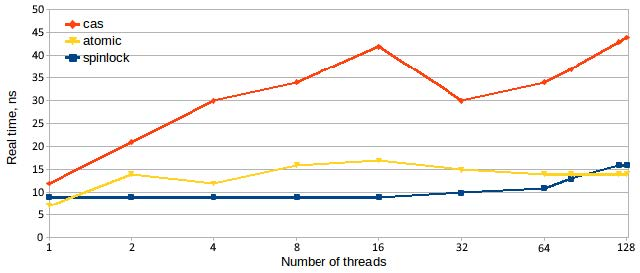
\includegraphics[width=0.9\textwidth]{content/2/chapter6/images/2.jpg}\\
图6.2 - 共享计数增量的性能:基于自旋锁、无锁(比较-交换,或CAS)和无等待(原子)
\end{center}

自旋锁已经做得很好了,性能明显优于比较-交换实现,并可以与无等待操作进行竞争。这里会有两个问题:首先,如果自旋锁的速度快得多,为什么不都使用自旋锁?其次,如果自旋锁这么好,为什么还需要原子操作(当然,除了锁实现的原子操作)?

第一个问题的答案可以归结为本节的标题,不同的问题使用不同的锁。自旋锁的缺点是等待的线程不断地使用CPU或“忙等待”。另一方面,等待系统互斥的线程大部分是空闲的(休眠)。如果需要等待几个周期,即增量操作的持续时间,那么忙碌等待也不错,比让线程进入睡眠状态要快得多。另一方面,如果锁定的计算包含多个指令,那么等待自旋锁的线程将浪费大量CPU时间,并剥夺其他工作线程访问所需的硬件资源的机会。总的来说,C++的互斥量(\texttt{std::mutex})或OS的互斥量通常会进行平衡,锁定一条指令的效率有点低,锁定一个需要几十纳秒的计算是可以的。如果需要持有锁很长时间(长是相对的,处理器很快,所以1毫秒是非常长的),这就打败了另一种选择。已经讨论了极端性能(以及极端实现性能的努力),因此大多数HPC开发者要么实现自己的快速锁来保护短计算,要么使用现成的库。

第二个问题,“锁还有其他的缺点吗?”让我们带着这个问题进入下一节。

\subsubsubsection{6.3.3\hspace{0.2cm}锁的和无锁的区别}

在讨论无锁编程的好处时,第一个点是“更快”。但这并不一定,如果针对特定的任务进行优化,锁的实现可以非常高效。但是,基于锁的方法还有其他缺点,不过这些缺点不依赖于实现。

最头痛的是可能出现死锁。当程序使用多个锁时,就会发生死锁,比如lock1和lock2。线程A拥有lock1,需要获取lock2。线程B已经拥有了lock2,需要获取lock1。两个线程都不能继续,而且都将永远等待,因为唯一可以释放它们所需锁的线程被锁阻塞了。

如果同时获得两个锁,总是以相同的顺序获得锁,就可以避免死锁。C++有一个用于此目的的函数\texttt{std::lock()}。但通常不能同时获得锁,当线程A获得lock1时,无法知道我们也需要lock2,因为该信息隐藏在由lock1保护的数据中。我们将在下一章讨论并发数据结构时看到一些例子。

如果不能获取多个锁,也许解决方案会尝试获取。然后,若不能获得所有的锁,那么释放已经持有的锁,以便其他线程可以获得。在我们的例子中,线程A持有lock1,它也会尝试获得lock2,但不会阻塞。大多数锁都有\texttt{try\_lock()},要么获得锁,要么返回false。后一种情况下,线程A释放lock1并试图再次锁定它们。这可能行得通,特别是在一个简单的测试中。但它自己也有危险,当两个线程不断地传递锁时,就会出现活锁。线程A有lock1,但没有lock2,线程B有lock2,放弃了它,得到了lock1,现在它不能再得到lock2了,因为线程A拥有了lock2。有一些算法可以获取多个锁,从而保证最终成功。但这可能要需要很长一段时间,并且算法也相当复杂。

解决多个锁的问题是互斥对象不能组合,不能将两个或多个锁组合成一个。

即使没有活锁和死锁的危险,基于锁的程序也会遇到其他问题。其中较为频繁和难以诊断的一种称为协同。可以在多个锁中发生,也可以只在一个锁中发生。协同看起来是这样的:假设有一个锁保护的计算。线程A目前拥有这个锁,并且正在对共享数据进行操作,其他线程正在等待。然而,这项工作并不是一次性的,每个线程都有许多任务要做,每个任务的一部分需要独占访问共享数据。线程A完成一个任务,释放锁,然后快速切换到下一个任务,直到它再次需要锁。锁释放了,其他线程都可以获得,但其他线程没完全醒,而线程A在CPU上,并没有睡。因此,线程A再次获得锁,只是因为竞争对手还没有做好准备。线程A的任务像车队中的卡车一样快速执行,而其他线程什么也做不了。

锁的另一个问题是,没有优先级的概念。持有锁的低优先级线程可以抢占需要相同锁的高优先级线程。因此,高优先级线程必须等待低优先级线程决定的时间,这种情况似乎与高优先级的概念不一致,这种情况有时称为优先级倒置。

既然已经理解了锁的问题并不局限于性能,那么看看无锁程序在相同的复杂性下会有怎样的表现。首先,在无锁程序中,至少有一个线程不被阻塞。最坏的情况是,当所有线程同时执行比较-交换(CAS)操作,并且原子变量的期望与当前值相同时,其中一个线程将看到期望值(因为唯一可以更改的方法是通过CAS操作)。其他线程将放弃它们的计算结果,重新加载原子变量,并重复计算,但是在CAS上成功的线程可以移动到下一个任务,这避免了死锁的可能性。如果排除了死锁和避免死锁的尝试,也就不必担心活锁。由于所有线程都忙于计算通向原子操作(如CAS)的路径,高优先级线程更有可能最先到达那里,并提交其结果,而低优先级线程更有可能使CAS失败,并重做其工作。类似地,提交结果的一次成功并不会使“获胜”的线程比所有其他线程有任何优势,准备先尝试执行CAS的线程就是成功的线程。这自然就消除了出现协同的可能。

无锁编程有什么不好呢?有两个主要的缺点。第一个是其优点的反面,即使CAS尝试失败的线程也会保持忙碌。这解决了优先级问题,但代价很高。在高争用的情况下,大量的CPU时间会浪费在重复工作上。更糟糕的是,这些为访问单个原子变量而竞争的线程,会从进行一些不相关计算的其他线程那里夺取CPU资源。

第二个缺点性质完全不同。虽然大多数并发程序都不容易编写或理解,但无锁程序的正确设计和实现都非常困难。基于锁的程序只需要保证构成单个逻辑事务的操作集都在锁下执行。当存在多个逻辑事务时,例如(而不是所有)共享数据对几个不同的事务来说是公共的,这就更难了。这就是提出多锁问题的原因。尽管如此,推断基于锁的正确性并不是那么困难。如果代码中有一段共享数据,就必须指明哪个锁保护该数据,并证明没有线程可以在不先获取该锁的情况下访问该数据。如果不是这样,那么就会出现数据竞争。如果满足了这些需求,就不会出现数据竞争(可能会出现死锁和其他问题)。

另一方面,无锁程序有无限多种数据同步方案。因为没有线程会暂停,所以无论线程执行原子操作的顺序如何,结果都必须是正确的。此外,如果没有明确的临界区,就得担心内存序和程序中所有数据的可见性,而不仅仅是原子变量。这里必须问问自己,有没有可能因为内存顺序要求不够严格,一个线程可以更改数据,而另一个线程可以看到这个数据的旧版本?

解决复杂性问题的通常方法是模块化和封装。将复杂的代码收集到模块中,每个模块都有一个定义良好的接口和一组明确的需求和保证,主要关注实现各种并发算法的模块。不过本书会有一个不同的方向,本章的其余部分将专门讨论适用于并发的数据结构。




































